\section{Experimental Setup}

\begin{figure}[t]
\centering
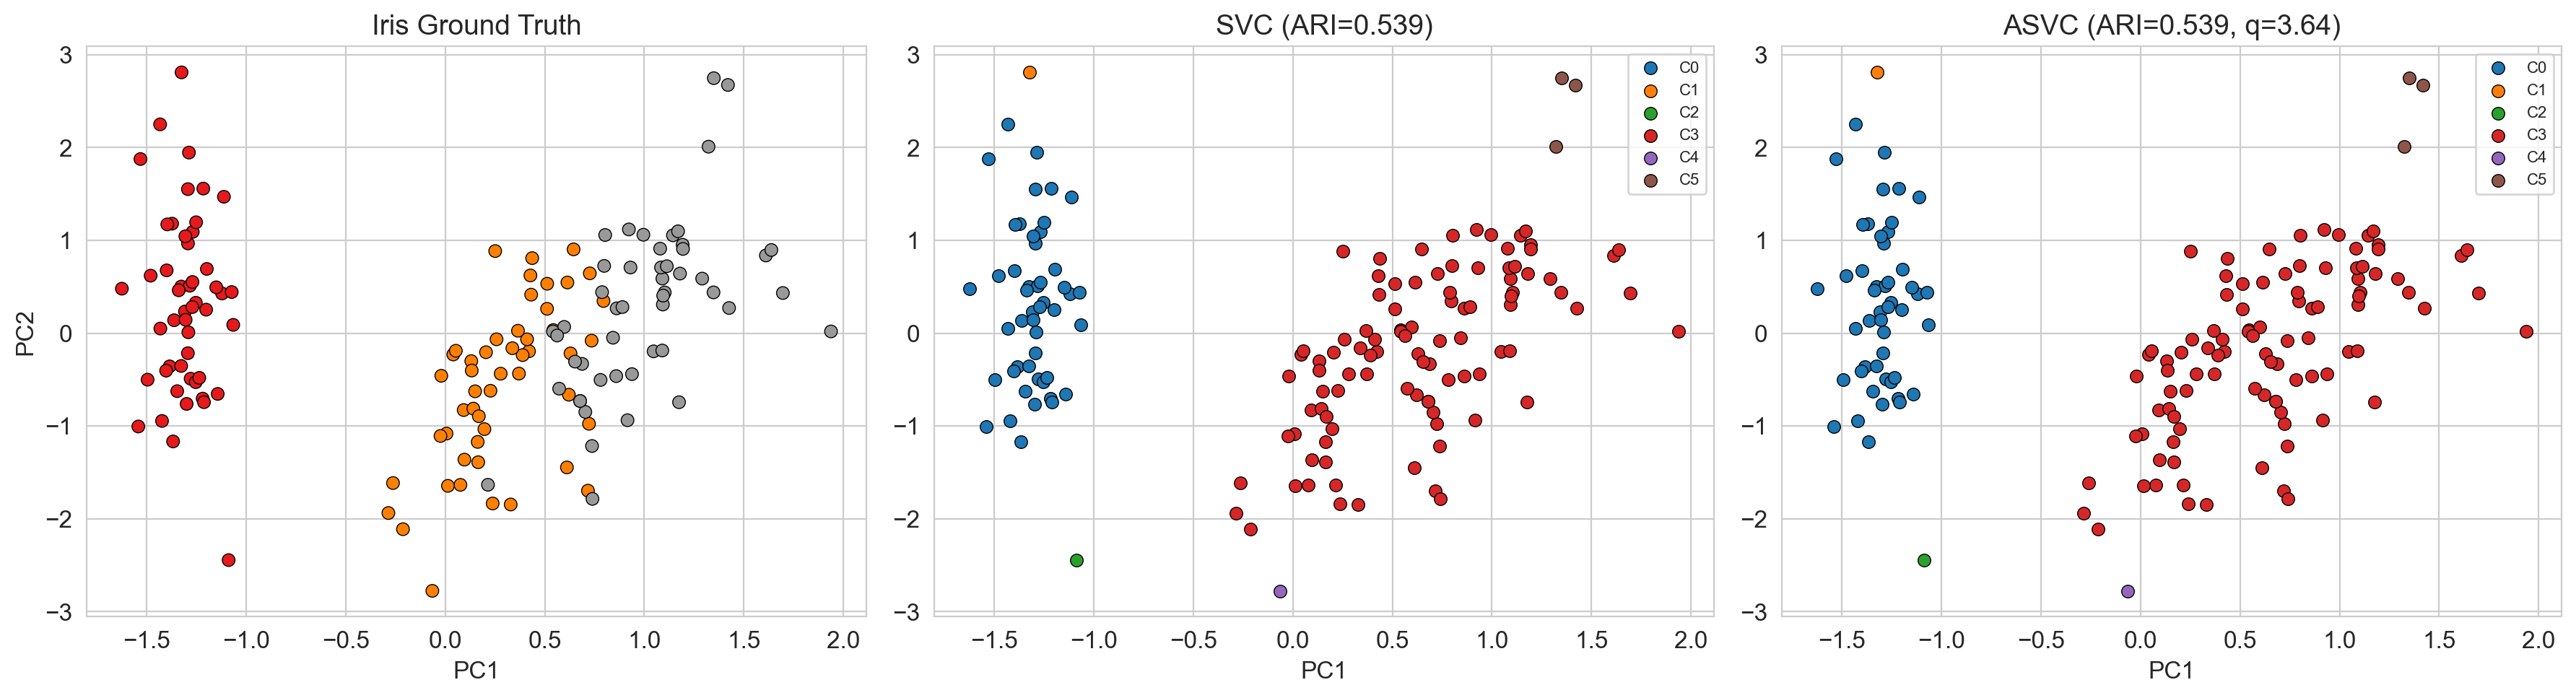
\includegraphics[width=\columnwidth]{fig/fig3_iris.png}
\caption{Clustering results on the Iris dataset (2D PCA). From left to right: ground truth labels, SVC clustering, and ASVC clustering. ASVC automatically selects appropriate parameters and produces meaningful cluster assignments without any label guidance.}
\label{fig:iris}
\end{figure}

\subsection{Datasets}

We use six synthetic datasets ($N=300$, 2D) spanning typical clustering challenges. All datasets are standardized to zero mean and unit variance.

\textbf{TwoMoons:} Generated via \texttt{make\_moons} (noise=0.08), two interleaving half-moons. Challenge: non-convex manifold separation.

\textbf{ConcentricCircles:} Generated via \texttt{make\_circles} (noise=0.05, factor=0.5), two concentric rings. Challenge: spatial interleaving of inner and outer circles with no density difference---simple distance-based methods cannot distinguish them.

\textbf{ThreeBlobs:} Generated via \texttt{make\_blobs} (cluster\_std=1.0), three isotropic Gaussian clusters. A standard baseline for verifying basic clustering capability.

\textbf{OverlappingGaussians:} Generated via \texttt{make\_blobs} (cluster\_std=2.0), three highly overlapping Gaussian clusters. Design goal: prevent the original SVC from finding any valid cluster boundary at any $q$ value.

\textbf{TwoMoonsNoisy:} Generated via \texttt{make\_moons} (noise=0.12), a high-noise TwoMoons variant with blurred boundaries.

\textbf{VaryingBlobs} (our construction): Three Gaussian clusters with equal sample sizes (100 each) but unequal variances ($\sigma\!=\![0.5,2.0,3.0]$), with inter-center distances $\approx$8. Design goal: DBSCAN inevitably fails because a single global \texttt{eps} cannot simultaneously accommodate all three scales, while SVC/ASVC can form size-adaptive hyperspheres for different clusters.

\subsection{Compared Methods}

\textbf{K-Means}~\cite{macqueen1967}: $k$ set to true cluster count, sklearn defaults (\texttt{n\_init=10}).

\textbf{DBSCAN}~\cite{ester1996}: \texttt{eps} and \texttt{min\_samples} selected via grid search optimizing ARI (note: uses labels; an unfair comparison).

\textbf{Spectral Clustering}~\cite{ng2002}: Normalized Laplacian, RBF kernel, cluster count set to ground truth.

\textbf{SVC (original)}~\cite{benhur2001}: Manually tuned $q$ (grid-searched per dataset), $C\!=\!1.0$. Uses label information for parameter tuning.

\textbf{ASVC (ours)}: $\nu\!=\!0.02$ fixed, $q\!=\!\texttt{auto}$ fully automatic. Does not use any label information.

\subsection{Evaluation Metrics}

\textbf{ARI}~\cite{hubert1985} (primary): $\in[-1,1]$, 1 = perfect agreement, 0 = random-level agreement. Auxiliary metrics: NMI~\cite{strehl2002}, Homogeneity/Completeness~\cite{rosenberg2007}.
